\documentclass[12pt]{article}
\usepackage[spanish]{babel}
\usepackage[margin=2.5cm]{geometry}
\usepackage{booktabs}
\usepackage{graphicx}
\usepackage{float}

% Tablas y figuras generadas por script/02_data_analysis.r.
\graphicspath{{../output/figures/}}

\title{Predicting Poverty: análisis descriptivo}
\author{Maria Jose Perez, Juan Manuel Lozano, Samuel Suárez Valle}
\date{\today}

\begin{document}
\maketitle

\section{Datos}

Se usa la muestra de entrenamiento de la GEIH 2018 (DANE): 543.103 personas
en 164.958 hogares. Un hogar es pobre cuando su ingreso per cápita de la
unidad de gasto (con arriendo imputado) es menor que la línea de pobreza de
su dominio. El 20,0\% de los hogares y el 25,1\% de las personas son pobres.

\section{Estadísticas descriptivas}

El Cuadro~\ref{tab:descriptivas} compara las medias de las características
de las personas pobres y no pobres. La diferencia es la media de los pobres
menos la de los no pobres, y el p-valor viene de una prueba $t$ de
diferencia de medias. Las variables de educación y de tenencia de vivienda
son dummies por categoría, así que su media es la proporción de personas en
esa categoría.

\begin{table}

\caption{\label{tab:descriptivas}Estadísticas descriptivas por condición de pobreza}
\centering
\begin{tabular}[t]{lrrrr}
\toprule
Variable & No pobres & Pobres & Diferencia & p-valor\\
\midrule
mujer & 0.525 & 0.541 & 0.016 & 0.000\\
afiliado\_salud & 0.941 & 0.906 & -0.035 & 0.000\\
ocupado & 0.508 & 0.304 & -0.204 & 0.000\\
educ\_ninguno & 0.041 & 0.093 & 0.052 & 0.000\\
educ\_preescolar & 0.026 & 0.040 & 0.014 & 0.000\\
\addlinespace
educ\_primaria & 0.232 & 0.343 & 0.111 & 0.000\\
educ\_secundaria & 0.166 & 0.230 & 0.064 & 0.000\\
educ\_media & 0.240 & 0.202 & -0.039 & 0.000\\
educ\_superior & 0.295 & 0.092 & -0.203 & 0.000\\
educ\_no\_sabe & 0.000 & 0.000 & 0.000 & 0.289\\
\addlinespace
vivienda\_propia\_pagada & 0.427 & 0.294 & -0.133 & 0.000\\
vivienda\_propia\_pagando & 0.041 & 0.016 & -0.025 & 0.000\\
vivienda\_arriendo & 0.353 & 0.414 & 0.061 & 0.000\\
vivienda\_usufructo & 0.145 & 0.159 & 0.014 & 0.000\\
vivienda\_sin\_titulo & 0.032 & 0.115 & 0.082 & 0.000\\
\addlinespace
vivienda\_otra & 0.001 & 0.001 & 0.001 & 0.000\\
Estrato1 & 3.122 & 2.126 & -0.996 & 0.000\\
tamano\_empresa & 2.152 & 0.642 & -1.510 & 0.000\\
anos & 35.651 & 27.303 & -8.347 & 0.000\\
meses\_empresa & 43.769 & 25.511 & -18.258 & 0.000\\
\addlinespace
horas\_trabajo\_semana & 45.421 & 41.735 & -3.687 & 0.000\\
cuartos\_hogar & 3.724 & 3.212 & -0.512 & 0.000\\
cuartos\_dormir & 2.341 & 2.203 & -0.138 & 0.000\\
arriendo\_estimado & 599617.307 & 277717.379 & -321899.928 & 0.000\\
prop\_edad\_trabajar & 0.856 & 0.731 & -0.125 & 0.000\\
\bottomrule
\end{tabular}
\end{table}


\section{Visualización}

Las figuras relacionan el ingreso per cápita con cada variable. La línea roja
punteada es la mediana de la línea de pobreza (\$280.072); la línea varía
por dominio, por lo que se usa la mediana como referencia.

\begin{figure}[H]
  \centering
  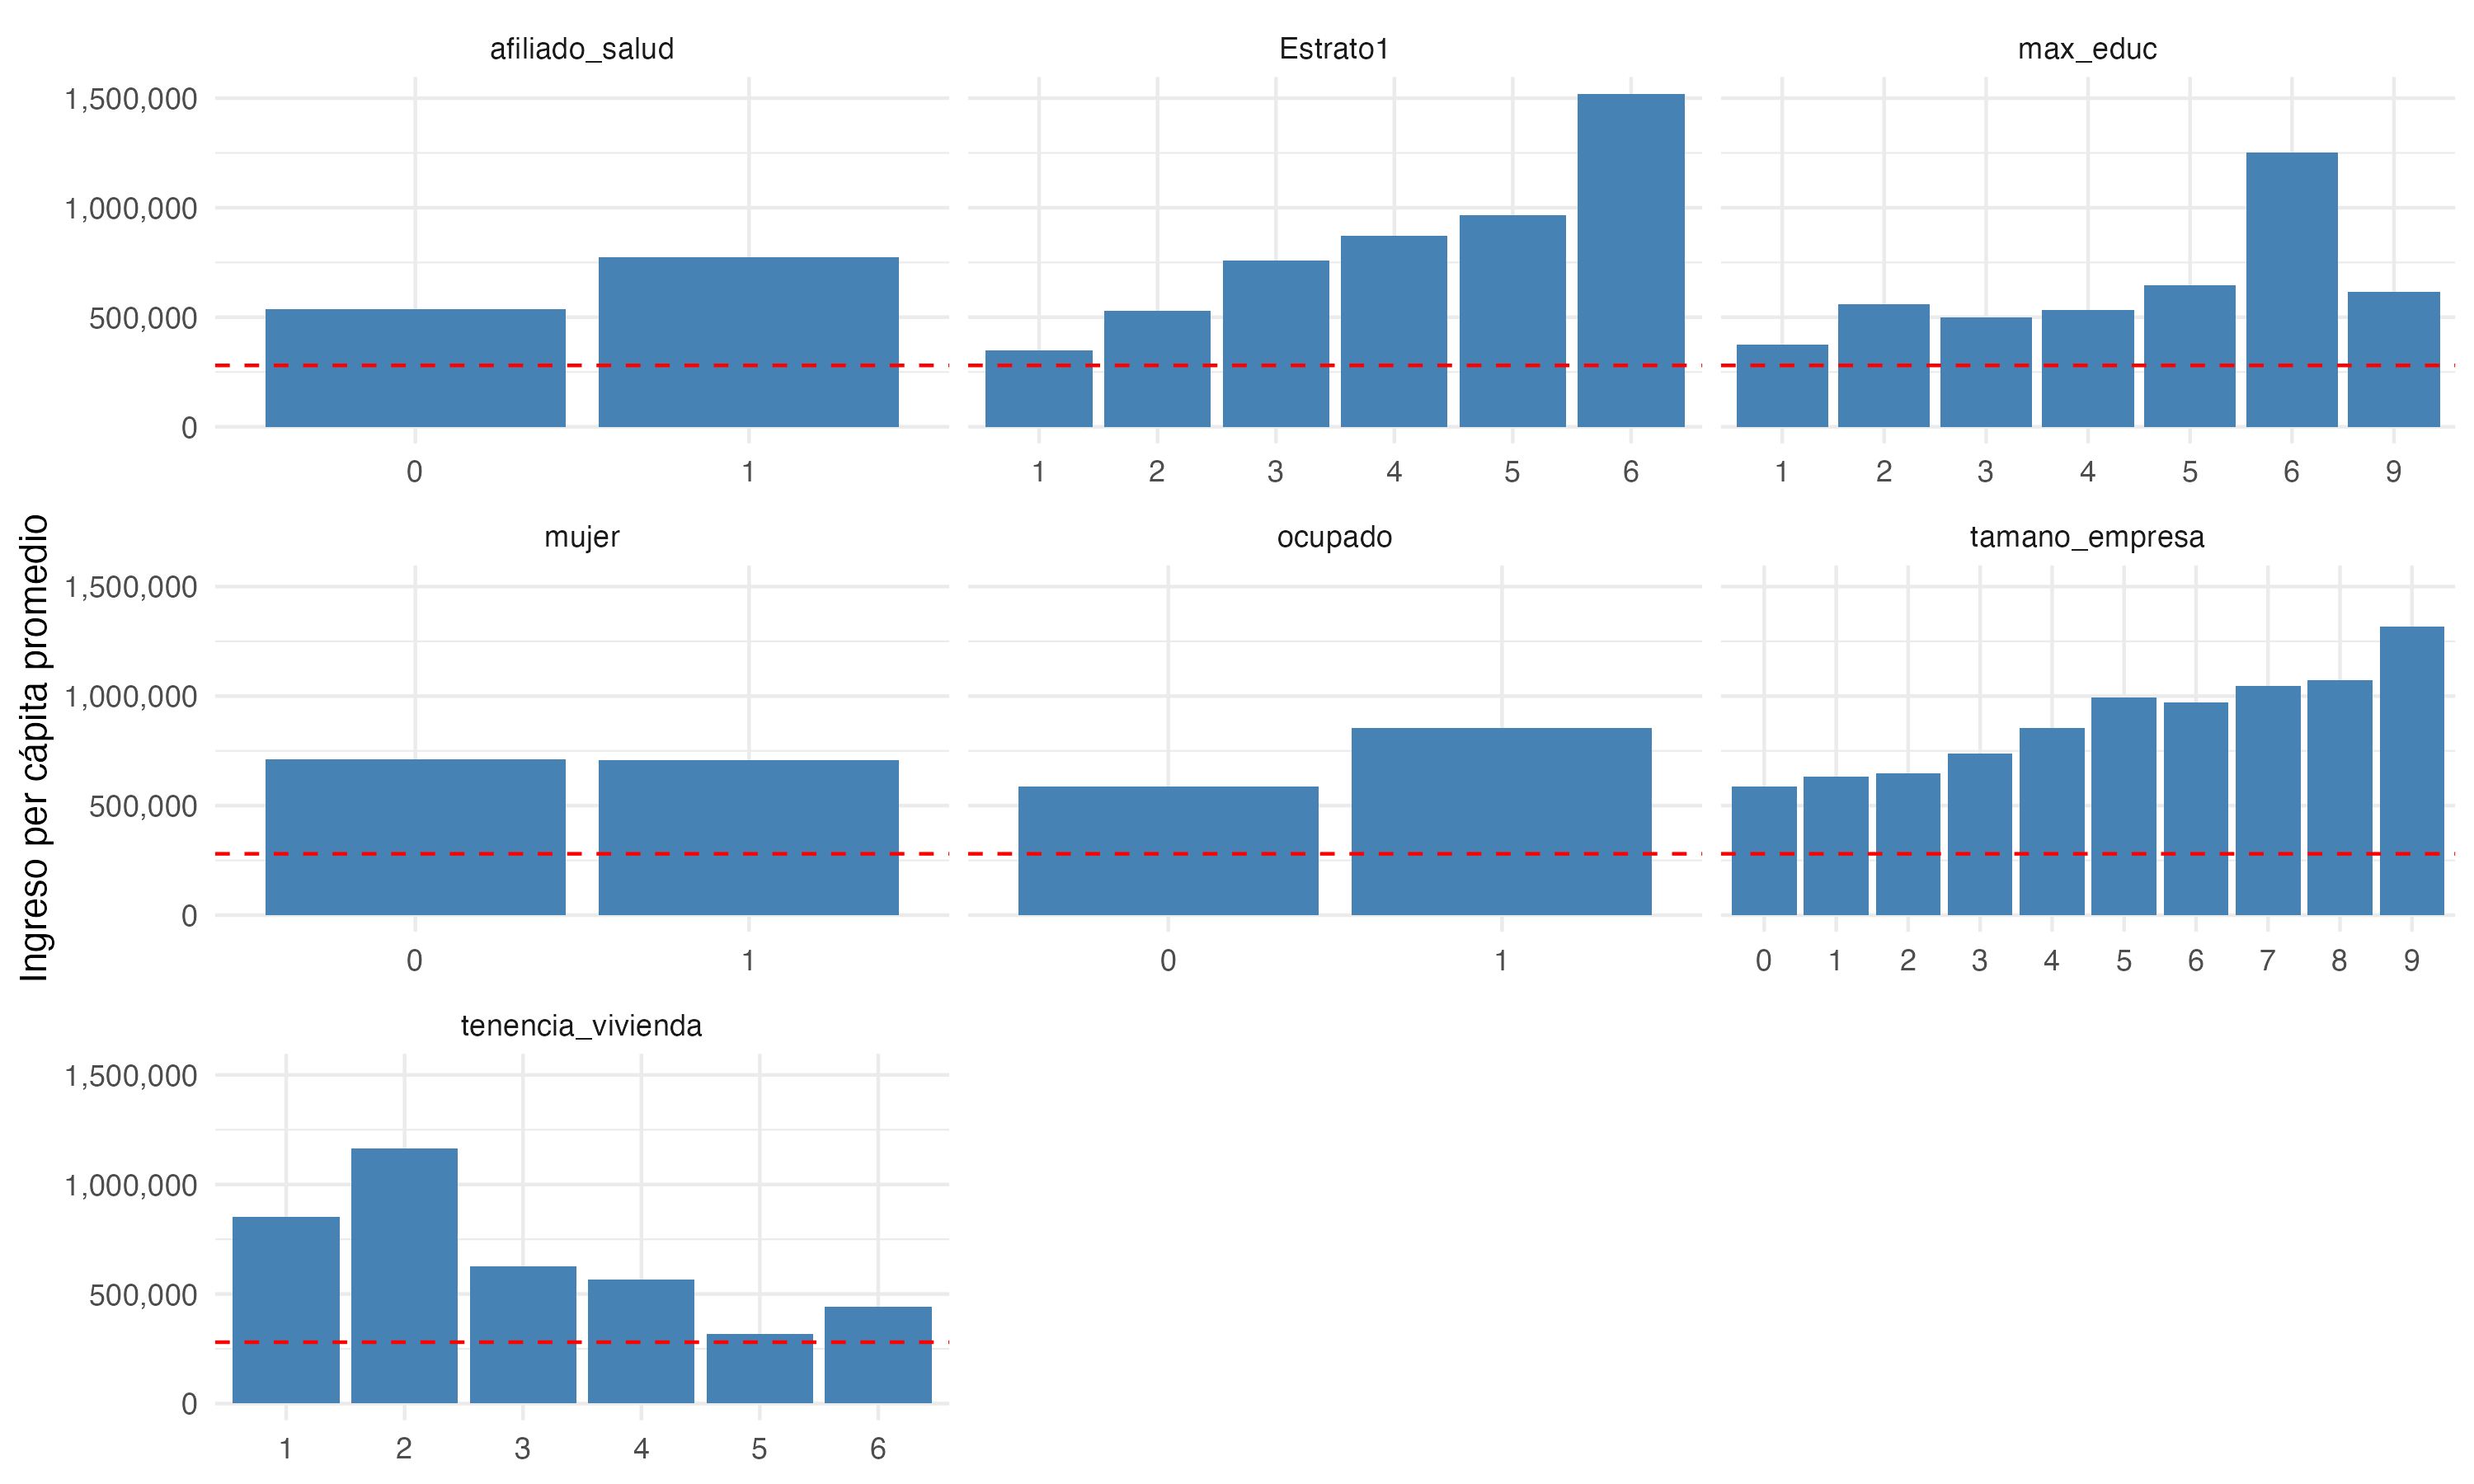
\includegraphics[width=\textwidth]{ingreso_dummies.png}
  \caption{Ingreso per cápita promedio por categoría de las variables
    dummies y categóricas.}
  \label{fig:dummies}
\end{figure}

\begin{figure}[H]
  \centering
  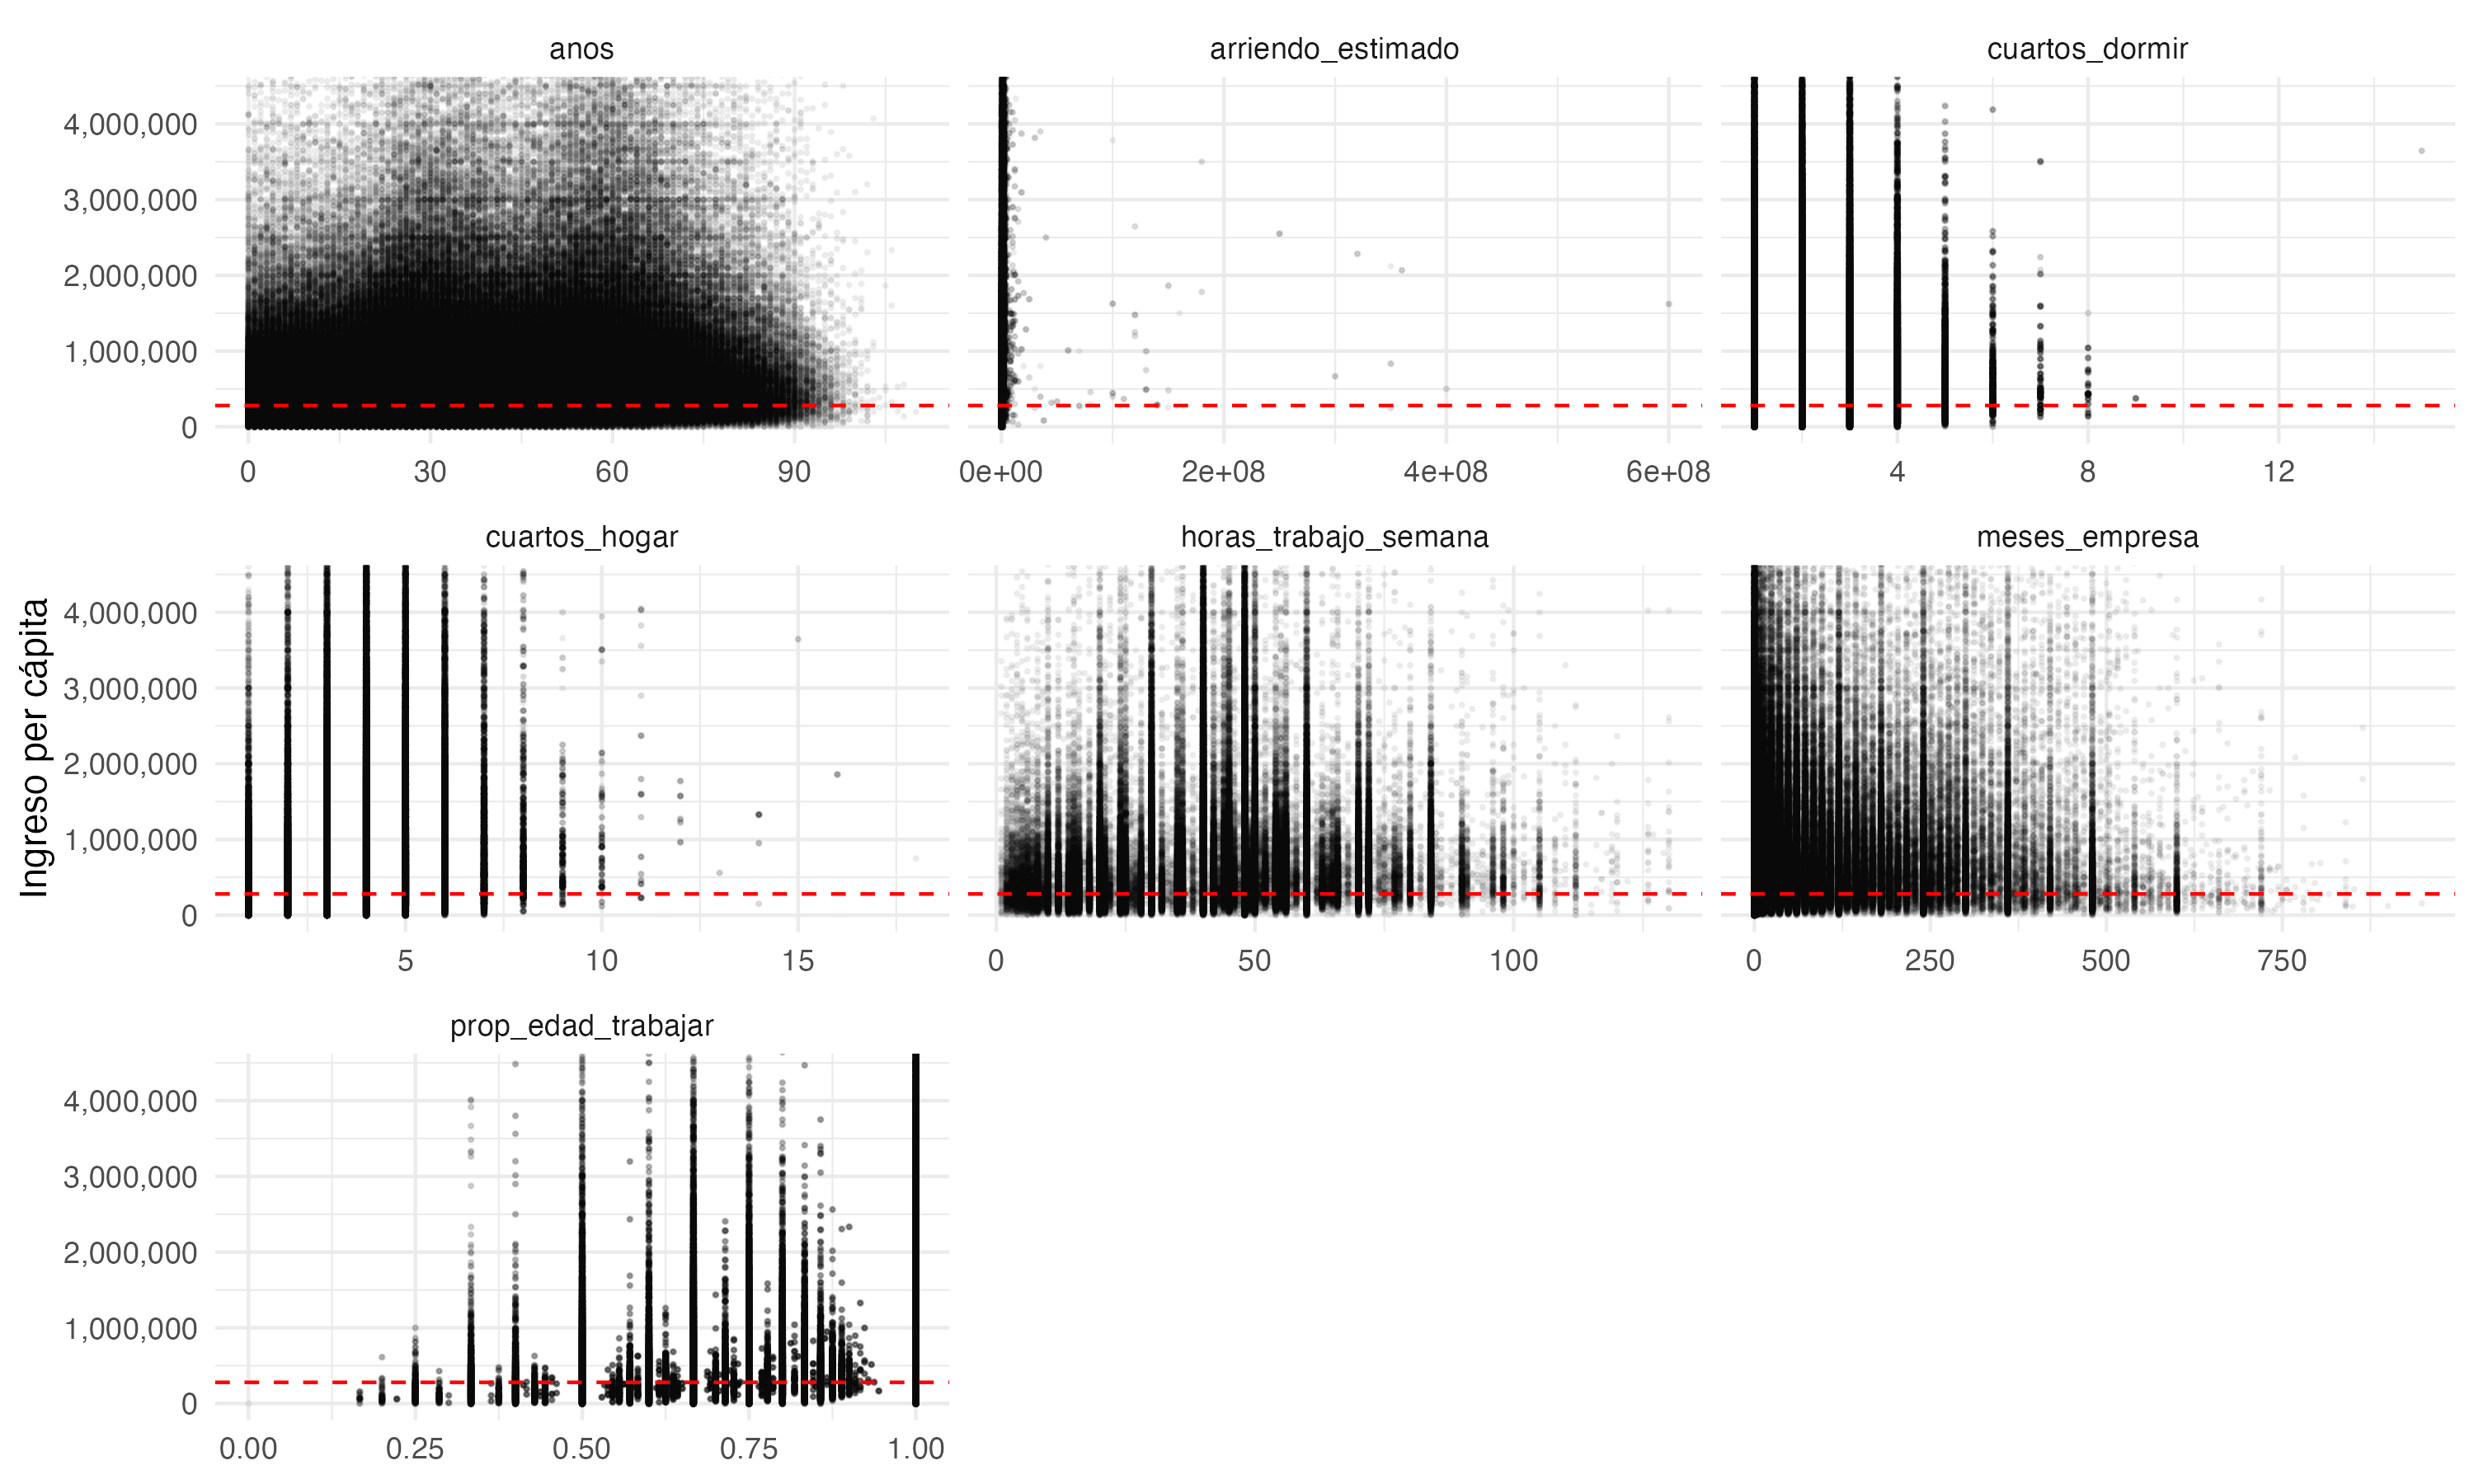
\includegraphics[width=\textwidth]{ingreso_continuas.png}
  \caption{Ingreso per cápita frente a las variables continuas. El eje $y$
    se corta en el percentil 99 del ingreso (\$4.400.000).}
  \label{fig:continuas}
\end{figure}

\end{document}
